% !TeX document-id = {c374cb94-c52b-488b-895c-d0d4efdafa72}
% !TeX spellcheck = en_US
% !TeX program=pdflatex
% !BIB program=biber

%%%%%%%%%%%%%%%%%%%%%%%%%%%%%%%%%%%%%%%%%%%%%%%%%%%%%%%%%%%%%%%%%%%%%%%
% Options for the class:
% 'fullpaper' if you are submitting a 6-page paper or
% 'abstract' if you are submitting a 2-page extended abstract.
% 'review' (is the default) will anonymize the submission and will add the review line numers.
% 'final' will add a mandatory footer on the titlepage which must contain the correct volume. This will be provided once the paper is accepted and everything is ready for publication. This footer is only necessary for full papers.
%%%%%%%%%%%%%%%%%%%%%%%%%%%%%%%%%%%%%%%%%%%%%%%%%%%%%%%%%%%%%%%%%%%%%%%
%\documentclass[fullpaper,final]{nldl}
\documentclass[fullpaper]{nldl}
%\documentclass[abstract]{nldl}

% Use the paper submission number
\paperID{Candidate \#11}
% defaults to current year plus one, or you can set it here (setting the year automatically updates the number of the conference)
\confYear{2024}
\type{Winter School Project Report}

%% Camera ready
% defaults to the current year count, or you can set it here
%\confNum{42}
% Replace 'V' with the provided number
%\vol{V}
%%%%%%%%%%%%%%%%%%%%%%%%%%%%%%%%%%%%%%%%%%%%%%%%%%%%%%%%%%%%%%%%%%%%%%%


%% Math
\usepackage{mathtools}

% Figures
\usepackage{graphicx}
\graphicspath{{Images/}}
\usepackage{todonotes}


%% Tables
\usepackage{booktabs}


%% Lists
\usepackage{enumitem}


% Algorithms
\usepackage{algorithm}
\usepackage{algorithmic}
\newcommand{\theHalgorithm}{\arabic{algorithm}}



%% Code
\usepackage{listings}
\lstset{
  basicstyle=\small\ttfamily,
  breaklines,
}

% References
\addbibresource{references.bib}


% Links and hyperlinks
\usepackage{hyperref}
\usepackage{url}
\hypersetup{
  pdfusetitle,
  colorlinks,
  linkcolor = BrickRed,
  citecolor = NavyBlue,
  urlcolor  = Magenta!80!black,
}
\usepackage[capitalise]{cleveref}
\newcommand\crefrangeconjunction{--}


% Replace with your title, authors and affiliation
\title{Exploring Generation of Optical Earth Observation Satellite Images with Various Denoising Diffusion Probabilistic Model Noise Schedulers}
%\author[1]{John Doe\thanks{Corresponding Author.}}
%\author[1,2]{Jane Doe}
%\affil[1]{Affiliation 1}
%\affil[2]{Affiliation 2}
%\affil[ ]{\texttt{\{john.doe, jane.doe\}@affiliation.com}}


\begin{document}
\maketitle

\begin{abstract}
Denoising diffusion probability models have become very good at generating realistic looking images using tricks like regularly adding noise following some scheduler, and using diffusion and neural networks to decode the noisy images back to noise-free images. The trained models can then generate new images similar to the images used in training. In this project, the theory behind the denoising diffusion models have been presented as well as giving an introduction into the dataset and network used. For training, three different noise schedulers, linear, cosine and sigmoid, have been used to train three different diffusion models to generate realistic Earth observation satellite images. The goal is to experiment and see if training with different noise schedulers yield different results. Using the SEN12MS summer season dataset as input, the models prove after 10 epochs of training to being able to generate close to realistic images without much hyperparameter tuning. They show similar image terrain in comparison to the real data, while producing minor differences in the samples.
\end{abstract}


\section{Introduction}
\label{sect:Intro}
Computer vision using artificial intelligence and machine learning to do image analysis have become a very important field for retrieving information in digital images, which quickly becomes very difficult to do manually by humans. There are lots of applications and domains where machine learning has shown great potential and results in image analysis, e.g. in medicine, remote sensing, biology, physics, and much more. Using machine learning opens up for more automation as there are normally a lot of images to analyze, and a lot of information and features to extract from these images.

Deep learning (DL) has been further used to enhance the learning of often advanced and intricate features in images, going past the limitations of earlier used methods. These deep models are more capable of handling complexities in images that are difficult to see otherwise. Using components like convolutional neural networks have shown very good results in being able to capture neighboring pixel contents in images. This is often the case with real world remote sensing images in the field of Earth observation (EO). Here, airborne and spaceborne sensors are used to obtain spectral and spatial information of the Earth's surface and atmosphere \cite{zhu2018review} for various applications. These types of applications often involve satellite images with various amount of spectral bands, often in the multi- and hyperspectral ranges with deep and complex features. As light is wavelength dependent, sensors capturing light at several wavelengths can obtain different information of objects in its field of view. Which then can be put together to give useful new information. DL methods have become very much used for a variety of EO applications like environmental monitoring, change and real-time detection, time-series processing, object classification, data fusion, and more~\cite{chen2023special}. 


\subsection{Objectives}
\label{subsect:Objectives}
The objective of this report is to study how denoising diffusion models can be used to generate images in the domain of remote sensing and EO. Several experiments will be performed with a focus on making the model learn how to generate images that are comparable to real life EO images. Three different noise schedulers will be experimented with, to see how different schedulers can affect the learning and predictions made by the network. This is somewhat similar to the work by Chen~\cite{chen2023importance}, but will not go as in-depth as this project is restricted to experimenting with different noise schedulers to generate images without as much hyperparameter tuning involved. 


\section{Literature Review}
\label{sect:Literature}
With the introduction of Generative Adversarial Networks (GANs)~\cite{goodfellow2014generative} and diffusion models~\cite{ho2020denoising}, it's possible to generate realistic and diverse images for a range of applications. While GANs are using two networks competing with each other to produce more and more realistic data and images, diffusion models utilize transformation of random noise and diffusion to generate samples. Diffusion models transform noise in images back to non-noisy images, as it captures patterns and complexities in the input data using trained neural networks. The trained diffusion models can then generate whatever image is desired after learning distributions in the training data. What separates diffusion models from GANs is the possibility of allowing more stable generation of samples through more control of the generation process. The user has the opportunity to give the trained model some parameters on how the generated images should be. Some examples of proved diffusion models using text to image are DALLE-2 and Stable Diffusion, where sentences or several words are given as input to produce desired images.

Generation of high-quality samples has also become attractive in remote sensing. Some attractive applications in remote sensing can be
\begin{itemize}
	\item Super-resolution~\cite{sebaq2023rsdiff,han2023enhancing}: Utilizing the diffusion properties to enhance the quality of low-resolution remote sensing images that could be used to improve applications like environmental monitoring and land cover classification.
	\item Cloud removal~\cite{jing2023denoising,meraner2020cloud,zhao2023cloud}: Utilizing multi-model satellite images like SEN12MS-CR~\cite{sen12mscr}, clouded and cloud-free images can be used with Denoising Diffusion Probabilisitc Models (DDPMs) to remove clouds of various thickness in optical images. Further improvements are also shown by implementing cloud heading. Removing clouds is an important application to make better images for other remote sensing applications where looking at the ground is important.
	\item Change detection~\cite{bandara2022ddpm}: Here the DDPM is trained on remote sensing images for extracting features, and then used as a pre-training for further change-detection. This shows to improve already existing change detection methods.
\end{itemize} 


\section{Methods}
\label{sect:Methods}
\subsection{Data}
\label{subsect:Data}
The dataset to be utilized in this project contains pre-processed multi-modal and mono-temporal satellite images collected by the Sentinel-1 and Sentinel-2 satellites, freely available data as a part of the European Space Agency's Copernicus mission, and Moderate Resolution Imaging Spectroradiometer (MODIS) land cover maps. This dataset is called SEN12MS \cite{Schmitt2019}, and was made to support the deep learning-based community developing approaches in remote sensing for doing common land cover tasks. It contains global data covering 252 (randomly sampled w.r.t. seasons) Regions of interest (ROI) across all inhabited continents recorded during all meteorological seasons throughout 2018. In this dataset: Sentinel-1 provides 2-band dual-pol synthetic aperture radar (SAR) images, Sentinel-2 provides processed cloud-free optical multi-spectral Top-of-atmosphere (L1C process level) 13 band images~\cite{web:S2_bands}, while MODIS provides processed four-band land cover patches from 2016. The full dataset contains 180~662 image patch triplets, each patch having size of 256~$\times$~256~$px^2$ at 10~m ground sampling distance.

For the purpose of this project, only Sentinel-2 images taken during the summer season are chosen for training the DDPM model. This season contains 65 globally distributed scenes/ROIs, with a total of 45~753 image patches~\cite{Schmitt2019}. Due to computational and time limits for this project only the three RGB bands, Red (665 nm), Green (560 nm) and Blue (490 nm) at 10~m pixel resolution, are used since these are the most important spectral bands for visualization.

Schmitt~\cite{Schmitt2019,ScmittSEN12MSdataset} also provides easy download of the full SEN12MS dataset, as well as supporting documents and a useful SEN12MS dataloader code for Python, which is used and modified to the needs of this project.


\subsubsection{Pre-processing of data}
\label{subsubsect:Preprocessing}
Sentinel-2 uses digital numbers as units for the optical bands. To make the pixel values manageable, each patch are first rescaled to physical surface quantities by dividing with 5000. This is due to that clouds often give higher pixel values since they are white, often making the rest of the scenes more darker than they have to be when further scaling and normalizations are applied (in case there are some clouds in the images or other higher intensities). 

To make the images better for human visualization, the RGB images are gamma adjusted by applying a power factor of 1/2.2~\cite{web:gamma}. The pixel intensities in each of the RGB bands are then further scaled to the [0, 255] range, which is more common in most digital images. For the images to be easier used in Python, the images are rearranged from dimension 3$\times$256$\times$256 (Bands, Height, Width) to 256$\times$256$\times$3 (Height, Width, Bands).

Lastly, some image transformations are applied; like rescaling to 128$\times$128 image sizes, adding random horizontal flip augmentations, and normalizing the images to pixel values in the -1 to 1 range better suited for the model to handle.


\subsection{Denoising Diffusion Probabilistic Model}
\label{subsect:DDPM}
The Denoising Diffusion Probabilistic Model (DDPM) theory is mostly based upon the work by Ho~\cite{ho2020denoising}, as well as the diffusion tutorial by Bianchi at the NLDL 2024 Winter School~\cite{bianchi2024DDPMtutorial}.


\subsubsection{Forward diffusion process}
\label{subsubsect:ForwardDiffusion}
The training set images are applied with some random Gaussian noise, $p(x_T):=\mathcal{N}(x_T,0,I)$, $T$ times ($T$ is a parameter) using a fixed Markov chain until the images are covered in noise, following the \textbf{forward diffusion} process with $T$ steps
\begin{equation}
	\label{eq:Forward}
	q(x_t|x_{t-1}) := \mathcal{N}(x_{t}; \sqrt{1-\beta_t}x_{t-1}, \beta_tI)
\end{equation}
seen in Figure~\ref{fig:DiffModelGraph}. For sufficiently large $T$ and with an appropriate choice of variance scheduler ($\beta_1$, ..., $\beta_T$), the image at step $T$ should be nearly an isotropic Gaussian.

\begin{figure}[h!]
	\centering
	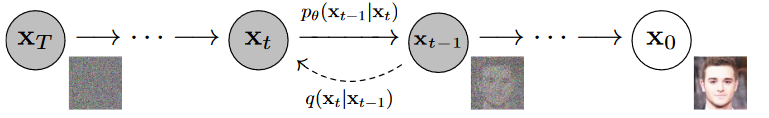
\includegraphics[width=1\linewidth]{DiffModelGraph.png}
	\caption{Directed graphical model with noisy image as input and predicted clean image as output. Source:~\cite{ho2020denoising}. \label{fig:DiffModelGraph}}
\end{figure}

In equation \ref{eq:Forward} there is a $\beta_t$ dependence in the forward diffusion process, which have to be calculated using a noise scheduler. There are various noise schedulers to choose from giving different beta mappings for stepping the model. Some of the most used schedulers are linear, sigmoid and cosine schedulers, having an impact on how quickly the noise is added to the images in terms of timesteps needed to fully cover the images in noise (like Figure 3 in~\cite{chen2023importance}).

A nice property is to rewrite the forward diffusion by setting $\alpha_t = 1 - \beta_t$ and $\bar{\alpha}_t = \sum_{i=1}^{t}\alpha_i$. Equation~\ref{eq:Forward} can then be changed to:
\begin{equation}
	\label{eq:Forward_alphas}
	q(x_t|x_0) = \mathcal{N}(x_{t}; \sqrt{\bar{\alpha}_t}x_0, (1-\bar{\alpha}_t)I).
\end{equation}
Now it is possible to sample $x_t$ at an arbitrary timestep $t$ in closed form~\cite{Schmitt2019} as
\begin{equation}
	\label{eq:sample_xt}
	x_t = \sqrt{\bar{\alpha}_t}x_0 + \sqrt{1 - \bar{\alpha}_t}z,
\end{equation}
given the noiseless input image $x_0$, and $z$ is the added isotropic Gaussian noise.


\subsubsection{Reverse denoising diffusion process}
\label{subsubsect:ReverseDenoise}
The noisy images will be fed as input to a neural network model together with the $t$ value, where the network will predict, approximating, the \textbf{reverse denoising} diffusion process 
\begin{equation}
	\label{eq:Reverse}
	p_{\theta}(x_{t-1}|x_t) := \mathcal{N}(x_{t-1}; \mu_{\theta}(x_t, t), \Sigma_{\theta}(x_t,t))
\end{equation}
to gradually denoise the images (see Figure~\ref{fig:DiffModelGraph}). The mean, $\mu_{\theta}$, and variance, $\Sigma_{\theta}$, needs to be handled computationally by a neural network, since they require the true data distribution $p(x)$ to be calculated analytically. $\Sigma_{\theta}$ can be set to untrained time dependent constants  $\Sigma_{\theta}=\sigma_t^2I=\tilde{\beta}_t$, while the mean needs to be computed by the neural network as
\begin{equation}
	\label{eq:Mean}
	\mu_{\theta}(x_t,t)=\frac{1}{\sqrt{\alpha_t}}(x_t - \frac{\beta_t}{\sqrt{1 - \bar{\alpha}_t}}\epsilon_{\theta}(x_t,t)),
\end{equation}
where $\epsilon_{\theta}(x_t,t)$ is the neural network predicted noise output. The output value for the reverse process at a given timestep $t$ can then be calculated as~\cite{Schmitt2019}:
\begin{equation}
	\label{eq:}
	x_{t-1} = \frac{1}{\sqrt{\alpha_t}}(x_t - \frac{\beta_t}{\sqrt{1 - \bar{\alpha}_t}}\epsilon_{\theta}(x_t,t)) + \tilde{\beta}_tz
\end{equation}


\subsubsection{Deep Learning Network}
\label{subsubsect:Network}
The network to be used for the diffusion model is a variant of the 2D U-Net~\cite{ronneberger2015u}. It takes in images of sizes 128$\times$128$\times$3, and outputs images of the same sizes. The architecture of the utilized U-Net is similar to Figure~\ref{fig:UNet}. The network has ResNet downsampling block layers, and corresponding same amount of ResNet upsampling block layers. Each downsampling layer shares features with its corresponding upsampling layer through skip-connections. As in Figure~\ref{fig:UNet}, each of the downsample and upsample layers contain two convolutional blocks followed by group normalization, attention, a ResNet block and finally a downsampling or upsampling block, respectively. Between the last downsampling and first upsamling layers, a middle layer is applied with a convolutional block, attention and another convolution.

\begin{figure}[h!]
	\centering
	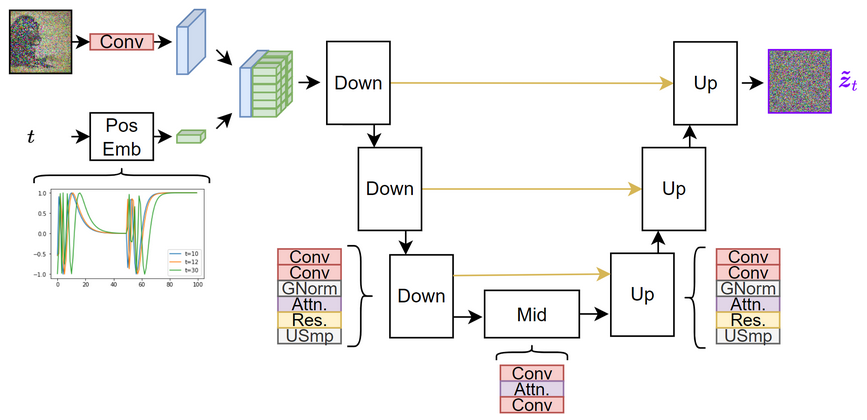
\includegraphics[width=1\linewidth]{UNet.png}
	\caption{U-Net components. Source:~\cite{bianchi2024DDPMtutorial}. \label{fig:UNet}}
\end{figure}

As mentioned in sect.~\ref{subsubsect:ReverseDenoise}, the network takes as input an image containing noise and the current timestep $t$ value. To encode the timestep information such that the network can properly handle it, sinusoidal position embedding is used as a transformer to encode the time position embedding of the noise in the input image at the current timestep given. This means that the parameters become shared accross time.

Given the noisy input, the network learns to predict the reverse process to produce images (optimally) without noise (as in Fig.~\ref{fig:DiffModelGraph}). With the predicted output and the noised images, the mean squared error (MSE) loss function is used to calculate the loss during training, which is logged and updated each step in the training process. Gradient descent is then applied, and the training process is repeated multiple times as the maximum number of training steps is a chosen parameter.

To set up the training process further; AdamW is used as the optimizer to update parameters, and a cosine learning rate scheduler with warm-up is applied to decrease the learning rate towards 0 following the cosine function. To follow the progress of the model training, Tensorboard is used to log the loss after each training step for easier visualization afterwards.


\subsection{Experiments}
\label{subsect:Experiments}
The work is done by utilizing existing code with DDPMs in the remote sensing domain to learn and generate realistic EO images, and compare the prediction quality for models with different noise schedulers. Smaller changes and additions are made to fit the specific needs for this project. The codes are available at \url{GITHUB_url}.

The DDPM code is mainly built upon the \textit{deonising-diffusion-pytorch} library~\cite{lucidrains2024} for training and sampling with the DDPM. This code will be referred to as the diffusion code from now on for simplification. For proper loading of the SEN12MS dataset, the initial dataloader provided by Schmitt~\cite{ScmittSEN12MSdataset} is used with an addition for doing the pre-processing mentioned in section~\ref{subsubsect:Preprocessing}.


\subsubsection{Training parameters}
\label{subsubsect:Training Params}
For all the experiments, a $T=500$ is used for adding the Gaussian noise. As in Figure~\ref{fig:UNet}, a three layer U-Net will be used to train the DDPM and make samples. For training; batch\_size=8 leading to about 5 720 batches with 8 samples each from the original 45 753 image patches, learning rate is set to 2e-5, to keep track of the Exponential Moving Average (EMA) version of the model EMA decay is set to 0.995, and amp=True is set to use mixed precision training. After every full epoch, save model and generate 25 sampling images. The only differences between the experiments are the noise schedulers: linear, sigmoid and cosine, giving in total three different main experiments. Other training parameters in the Trainer-function are kept as initialized in the function. The experiments are all run using 1 GPU, \textit{num\_workers=0} and training for 11 epochs.


\section{Results}
\label{sect:Results}
\subsection{Failed experiments}
\label{subsect:Res-Failed}
For a first and separate experiment, the Hugging Face's Diffusers library~\cite{von-platen-etal-2022-diffusers} tutorial on how to train diffusion models with PyTorch and the Diffusers library is tested.

For this experiment, linear and cosine beta-schedulers are tested to check the DDPM implementations with this code. The same SEN12MS dataset is used, and the same dataloader.


\subsubsection{Cosine noise scheduler}
\label{subsubsect:Res-cosine_fail} 
Using a cosine noise scheduler, the code is run for 33 epochs giving samples seen in Figure~\ref{fig:Failed-cosine}. Each 10th epoch produce 5 samples, and in the figure the samples produced after 10 and 30 epochs are shown row-wise. Completing one training epoch would take around 52 minutes.
\begin{figure}[h!]
	\centering
	\subfloat{
\includegraphics[width=1\linewidth]{Failed_experiments/cosinebeta_e9.png}}\\
	\subfloat{
\includegraphics[width=1\linewidth]{Failed_experiments/cosinebeta_e29.png}}
	\caption{Row-wise samples produced after 10 and 30 epochs of training with cosine noise scheduler. \label{fig:Failed-cosine}}
\end{figure}


\subsubsection{Linear noise scheduler}
\label{subsubsect:Res-linear_fail} 
Using a linear noise scheduler, the code was run for 50 epochs giving samples seen in Figure~\ref{fig:Failed-linear}. This figure shows the samples produced after 10, 30 and 50 epochs. Completing one training epoch would take around 52 minutes her as well.
\begin{figure}[h!]
	\centering
	\subfloat{
\includegraphics[width=1\linewidth]{Failed_experiments/linearbeta_e9.png}}\\
	\subfloat{
\includegraphics[width=1\linewidth]{Failed_experiments/linearbeta_e29.png}}\\
	\subfloat{
\includegraphics[width=1\linewidth]{Failed_experiments/linearbeta_e49.png}}
	\caption{Row-wise samples produced after 10, 30 and 50 epochs of training with linear noise scheduler. \label{fig:Failed-linear}}
\end{figure}


\subsection{Successful experiments}
\label{subsect:Res-exps}
For each of the three noise schedulers, after each epoch of training there are 25 samples produced and saved together with the model. In this section, some of the samples produced after 1 and 10 epochs are shown for each of the noise schedulers. Figure~\ref{fig:linear} shows some of the samples that are produced training with the linear noise scheduler, Figure~\ref{fig:cosine} shows some of the samples that are produced training with the cosine noise scheduler, and Figure~\ref{fig:sigmoid} shows some of the samples that are produced training with the sigmoid noise scheduler.

\begin{figure}[h!]
	\centering
	\subfloat[Epoch 1]{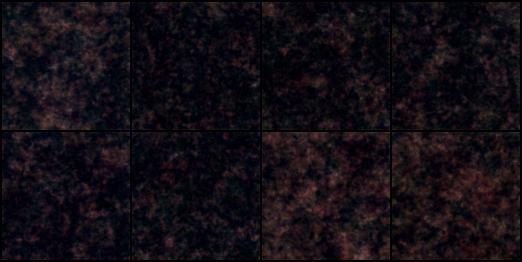
\includegraphics[width=1\linewidth]{linear-e1.png}}\\
	\subfloat[Epoch 10]{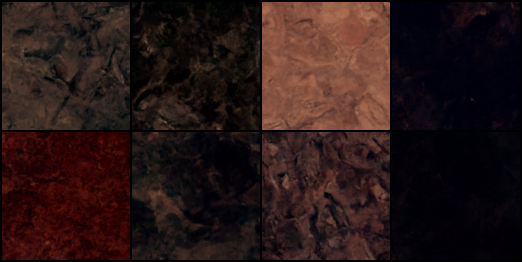
\includegraphics[width=1\linewidth]{linear-e10.png}}
	\caption{Samples produced after 1 and 10 epochs of training with linear noise scheduler. \label{fig:linear}}
\end{figure}

\begin{figure}[h!]
	\centering
	\subfloat[Epoch 1]{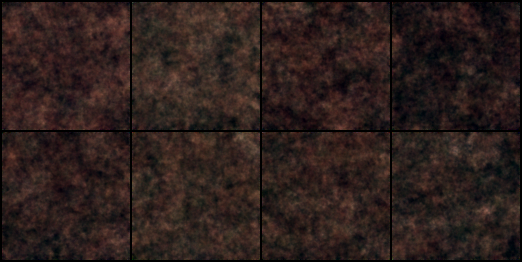
\includegraphics[width=1\linewidth]{cosine-e1.png}}\\
	\subfloat[Epoch 10]{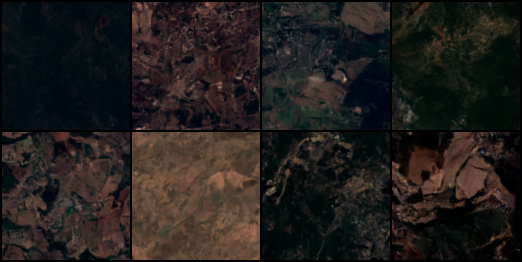
\includegraphics[width=1\linewidth]{cosine-e10.png}}
	\caption{Samples produced after 1 and 10 epochs of training with cosine noise scheduler. \label{fig:cosine}}
\end{figure}

\begin{figure}[h!]
	\centering
	\subfloat[Epoch 1]{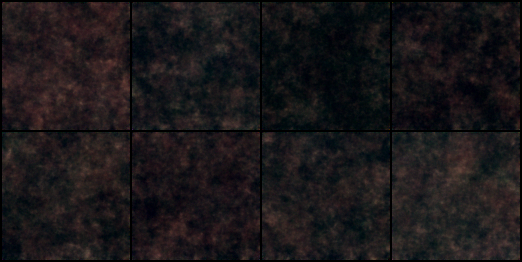
\includegraphics[width=1\linewidth]{sigmoid-e1.png}}\\
	\subfloat[Epoch 10]{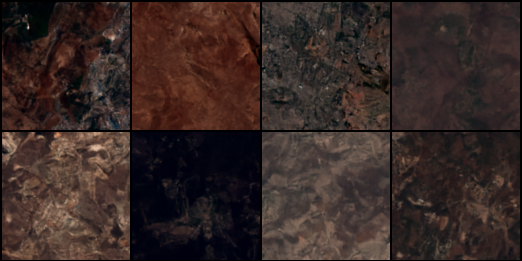
\includegraphics[width=1\linewidth]{sigmoid-e10.png}}
	\caption{Samples produced after 1 and 10 epochs of training with sigmoid noise scheduler. \label{fig:sigmoid}}
\end{figure}


\subsubsection{Training loss}
\label{subsubsect:Res-Loss}
The training loss curves for the three noise schedulers after 11 epochs of training are shown in Figure~\ref{fig:losses} on a log-scale per training step.
\begin{figure*}[t!]
	\centering
	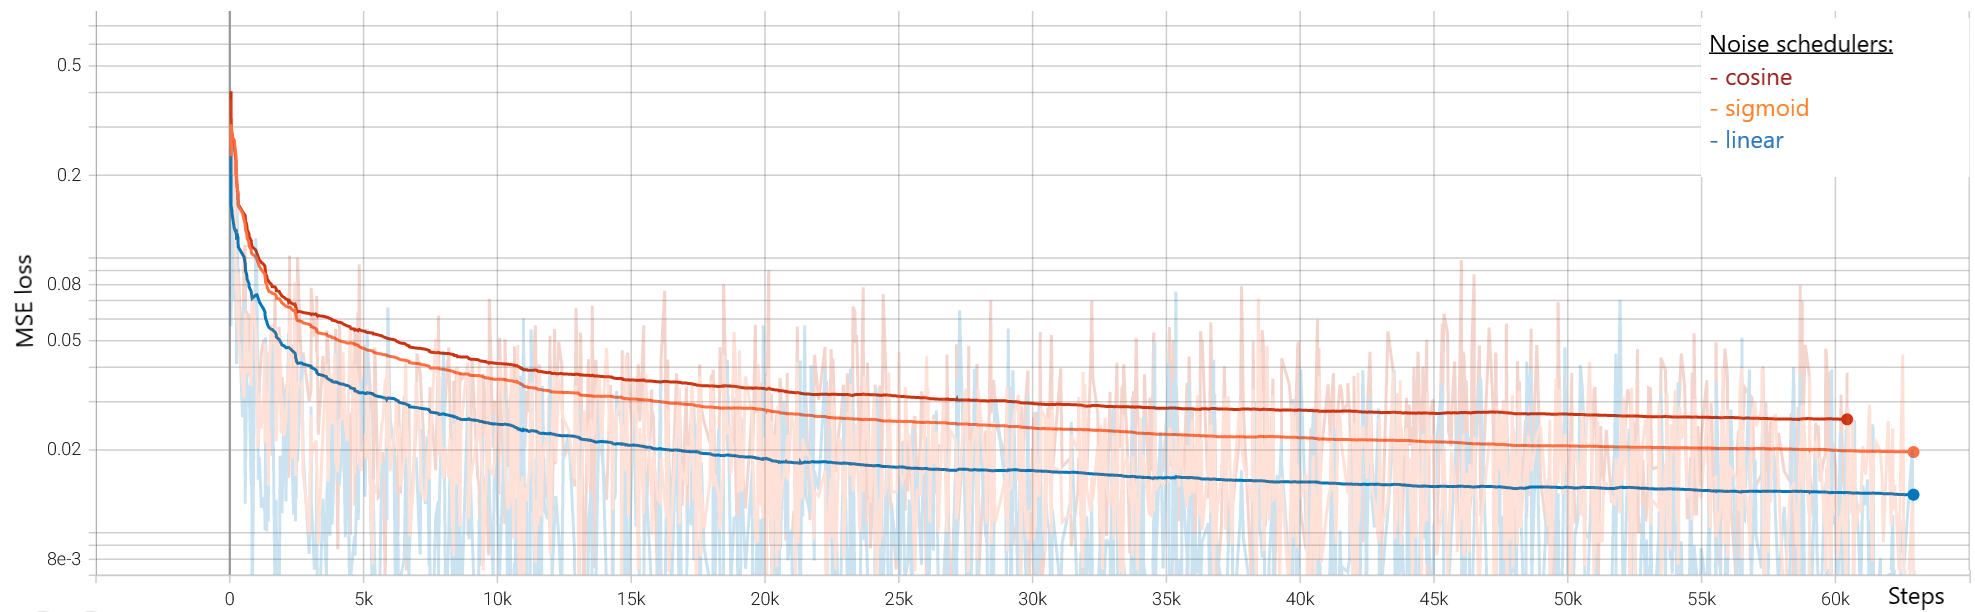
\includegraphics[width=1\linewidth,height=0.15\textheight]{Loss_curves.png}
	\caption{MSE loss curves for the three noise schedulers: linear (blue), sigmoid (orange) and cosine (burgundy). \label{fig:losses}}
\end{figure*}


\section{Discussion}
\label{sect:Discussion}
In Figure~\ref{fig:real_grid} there are some of the input images from the SEN12MS dataset to be used as a reference for what the DDPM is predicting.
\begin{figure}[h!]
	\centering
	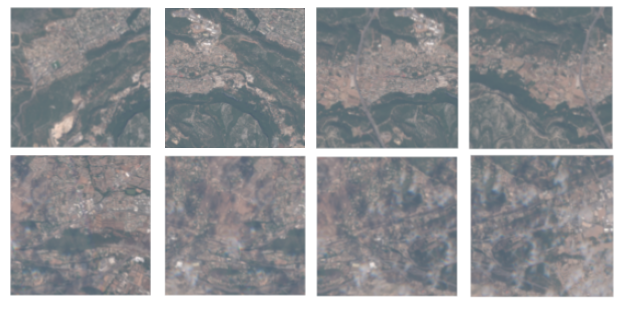
\includegraphics[width=1\linewidth]{real_grid_copy.png}
	\caption{Some examples of how the training data looks like from the SEN12MS dataset. \label{fig:real_grid}}
\end{figure}

As another reference, produced work by Adamiak~\cite{adamiak2023GenAI} is also compared with as the same denoising-diffusion-pytorch library have been used to train a diffusion model. The main difference is the dataset, which in this case is another satellite dataset containing mostly rivers, mountains and forests, called AID, here used for educational purposes to show how diffusion models work by generating artificial mountains. Some of the presented results achieved after 8 hours of training are shown in Figure~\ref{fig:ref_grid}.
\begin{figure}[h!]
	\centering
	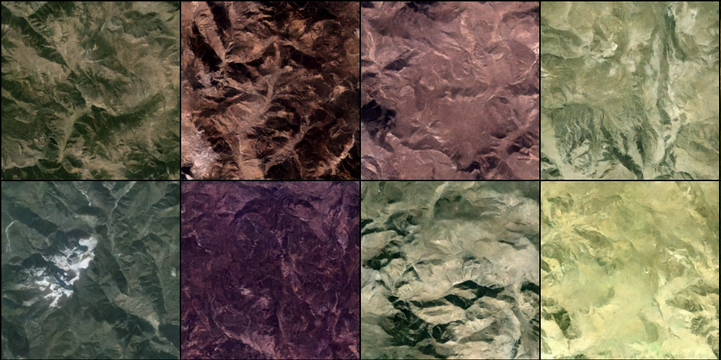
\includegraphics[width=1\linewidth]{reference_grid.png}
	\caption{Some of the presented results in~\cite{adamiak2023GenAI} for generating artificial mountains using same diffusion library as used in this report. \label{fig:ref_grid}}
\end{figure}


\subsection{Failed experiments}
\label{subsect:Failed Experiments}
\subsubsection{Idea 1}
\label{subsubsect:Idea1}
The original thought for this project was to use another dataset called SEN12MS-CR~\cite{sen12mscr}, which is a similar dataset to SEN12MS. The SEN12MS-CR dataset is patch-wise co-registered with the SEN12MS and contains Sentinel-1, and Sentinel-2 cloudy and cloud-free images used mainly for cloud removal in optical cloudy images. The idea was to use this SEN12MS-CR dataset and DDPMs to learn cloud removal~\cite{jing2023denoising}.

The DDPM cloud removal became to much to do and train, both due to the amount of data which required a lot of time and computational power leading to a smaller training set to be used, and struggles with making the model to do the DDPM cloud removal properly.


\subsubsection{Idea 2}
\label{subsubsect:Idea2}
From the DDPM cloud removal idea, some changes were made: First going to the SEN12MS dataset, reducing the amount of data to one season only, and only using Sentinel-2 RGB images would make it possible to learn the DDPM model to generate optical RGB images.

Two similar scripts were found for doing DDPM; the Hugging Face diffusion tutorial and the denoising-diffusion-pytorch model. The results from the Hugging Face diffusion is shown in section~\ref{subsect:Res-Failed}, showing that the code did not work properly. With the cosine noise scheduler, training for 30 epochs did not produce good samples as seen in Figure~\ref{fig:Failed-cosine}. With the linear noise scheduler, there might be indications of better samples when getting to 50 epochs in Figure~\ref{fig:Failed-linear}.

Simultaneously, the denoising-diffusion-pytorch model was also tested, and it showed better results in shorter time. Using the Hugging Face diffusion model, one epoch would take around 52 minutes. By the evolution of the produced samples with the linear nois scheduler, the model might need 80+ epochs to produce good or better results, leading to at least 70 hours of training to reach 80 epochs, after some calculations. This is why the Hugging Face diffusion model was set aside, and the denoising-diffusion-pytorch model was used in the end.


\subsubsection{Evaluation}
\label{subsubsect:Eval}
For evaluation of the sample quality by the model, the Frechet Inception Distance score (FID) was originally thought of since this is an often used metric for evaluating the quality of produced images by generative models. It is already implemented in the diffusion library, so it is easy to implement into the training of the models. Calculating the FID during training was after some consideration dropped due to a couple of reasons. 

To do proper and robust FID calculations, the model requires a lot of generated samples leading to a very big increase in time. First a smaller amount of samples were tested to see if using a small number of generated samples could be enough to get some usable quality estimate. This proved not to work. With the small amount of generated samples the time added to training was not too much, but the FID scores produced were too high, leading to an error in the program. This is ideally something that would be used for this type of task for quality check, but was decided to be removed due to time constraints for this project.


\subsection{Experiments}
All of the three main experiments with the diffusion library took around 13-14 hours to train for 11 epochs with the full summer season data from SEN12MS. In terms of number of epochs, this is slower than the first failed experiments mentioned in section~\ref{subsect:Res-Failed}. By comparing all the image samples produced in~\cref{fig:Failed-cosine,fig:Failed-linear,fig:linear,fig:cosine,fig:sigmoid}, the failed experiments clearly produce worse samples. The diffusion code clearly produces better images after 1 epoch with some recognizable terrain structures with reasonable colors considered it is produced after 1 epoch of training. The failed experiments did not show any sort of terrain structures until around 30 epochs, and there the colors are not correct. 

From the diffusion results in~\cref{fig:linear,fig:cosine,fig:sigmoid}, there clearly are improvements between epoch 1 and 10. Like the images in Figure~\ref{fig:ref_grid}, the produced samples are still not perfect in the case that we still can see that these are synthetic images. It's possible to see that the samples are terrain images with different environments and backgrounds. There are still some colors that are off, but the diffusion model is showing good promise of producing real looking high-quality images. They might need more training time to get even better results, as 10 epochs are not that much. But the preliminary results shows promise.

Comparing the samples with the real images from SEN12MS in Figure~\ref{fig:real_grid}, there are some brightness differences separating them. This is just due to some plotting and saving differences, as the structures between these images are the most important in this case. The terrain structures look not that far from each other for several of the samples produced by the diffusion model. For the terrain with the linear noise scheduler trained model (Fig.~\ref{fig:linear}), there are perhaps more color mismatch compared to the other noise schedulers. The terrain is also less prominent and clear compared to the others, looking like this one might need more epochs to train to catch up to the others.

The terrain in the cosine (Fig.~\ref{fig:cosine}) and sigmoid (Fig.~\ref{fig:sigmoid}) images looks very similar to each other. What separates the most could be the colors in some of the samples where a few of the sigmoid samples have some orange colors that does not seem to fit with the real life images. The cosine samples might look more realistic in the choice of coloring for the terrain. But they are both more stable and more realistic looking than the referenced images~\cite{adamiak2023GenAI}.

Since these experiments are not as advanced as~\cite{chen2023importance}, the datasets used are different, and FID calculations are missing in this project, it is difficult to properly compare results with the article. Th noise schedulers used are also a bit different in the article as compared to this project. But looking at Table 3 with FID scores for 128$\times$128 image sizes in the article, the best results are achieved with the sigmoid noise scheduler. This seems to be somewhat comparable when looking at the loss curves in Figure~\ref{fig:losses}. There, all three loss curves are quite similar with little difference between them (on log-scale) when applying some clever smoothing weight (applied with Tensorboard) as they are all flattening out within 0.01 and 0.03 with the MSE loss. Without the smoothing, there are more fluctuations per step which can be seen faintly in the background, so the smoothing is applied to see the overall loss trend for each noise scheduler. Sine the loss curves are on log-scale, they look to be flattening out more and more with each epoch of training. This does perhaps not correlate very well with the produced samples for the noise schedulers, as linear produced samples seems a little worse than the other two. But this is based upon direct visualization of the images, which might not be what the model have learned during training as seen by the loss curves. The shown produced samples might not be the best representative wise either.


\section{Conclusion}
\label{sect:Conclusion}
In this project, two different DDPM models have been presented and used to train and produce realistic EO terrain images using the SEN12MS dataset. The first did not produce reasonable results, and was dropped. The second showed good improvements from epoch 1 to 10 using three different noise schedulers in separate training for comparison between the three trained diffusion models. As the linear scheduler looks to be a bit behind in quality, cosine and sigmoid schedulers produce similar results, with cosine looking to be a little bit better and concise in its predictions and sampling of new images. This is again based upon looking at the produced samples. Further training with all three schedulers should give even better results if experimented with more, as the loss curves shows some stable tendencies but still goes down.


\subsection{Future work}
\label{subsect:Future}
As mentioned earlier in the report, there should optimally be more evaluation metrics to further evaluate the quality of the generated images. Which is why a future work could involve applying metrics like the FID score between the generated and real images.

Expanding the experiments like in~\cite{chen2023importance} could also be further explored, by adding more experiments like using other image sizes, adding input scaling and parameter tuning.

Other types of noise other than Gaussian could also be tested, like Perlin noise showing good results for terrain generation~\cite{jain2023Perlin} in the domain of remote sensing.

It is also possible to go back to the cloud removal with the SEN12MS-CR dataset now that there is a functional DDPM model ready for use on similar data.


\section*{Recommendations}
Future winter schools topics could be:
\begin{itemize}
	\item Dimensionality reduction
	\item Reinforcement learning
	\item Image inpainting
	\item Representation learning
\end{itemize}

\printbibliography

%\appendix

\end{document}
